\section{tweedledum}
\begin{frame}{induction}  
  ABC 
\end{frame}
\begin{frame}{compilation flow}
  \begin{figure}[htbq]
    \centering
    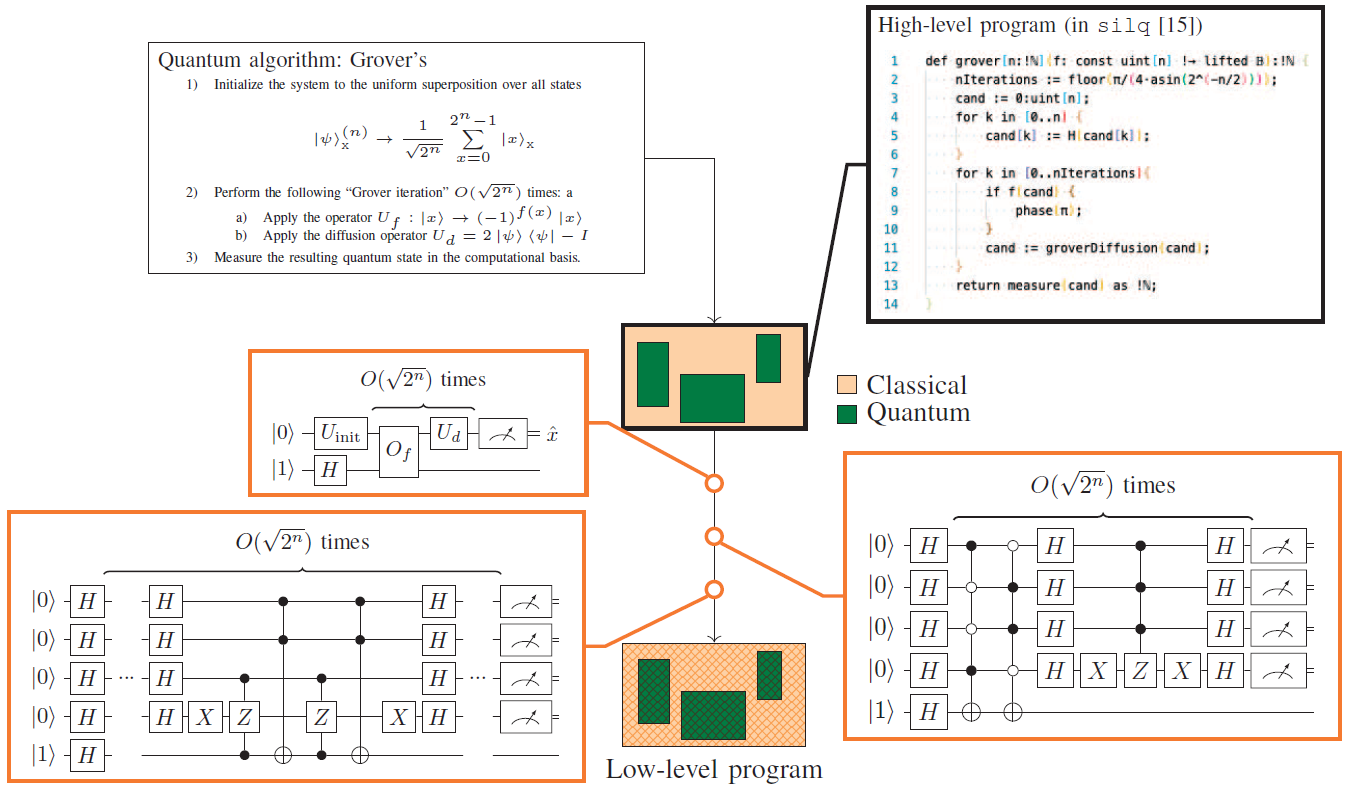
\includegraphics[width=0.8\textwidth]{figure/work_flow.png}
    \caption{compilation flow overview} 
    \label{fig-compilation}
  \end{figure}
\end{frame}
\begin{frame}{flexibility}
  \begin{figure}[htbq]
    \centering
    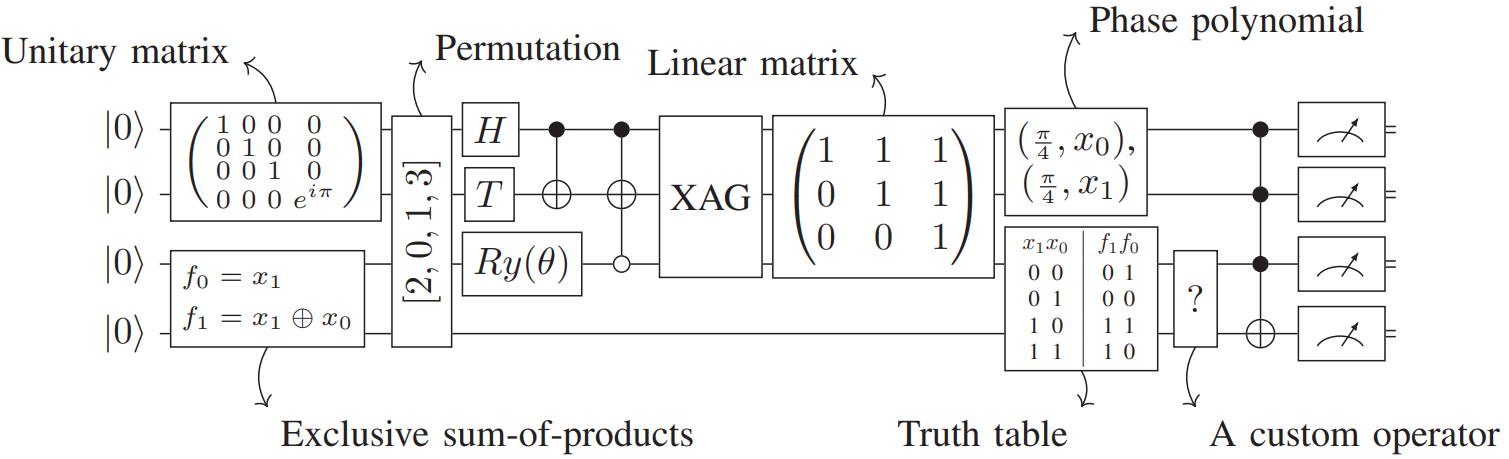
\includegraphics[width=0.9\textwidth]{figure/flex.png}
    \caption{tweedledum's IR flexibility} 
    \label{fig-flex}
  \end{figure}
\end{frame}
\begin{frame}{synthesis}
  \begin{itemize}
    \item 
  \end{itemize}  
\end{frame}
\begin{frame}{synthesis}
  \begin{figure}[htbq]
    \centering
    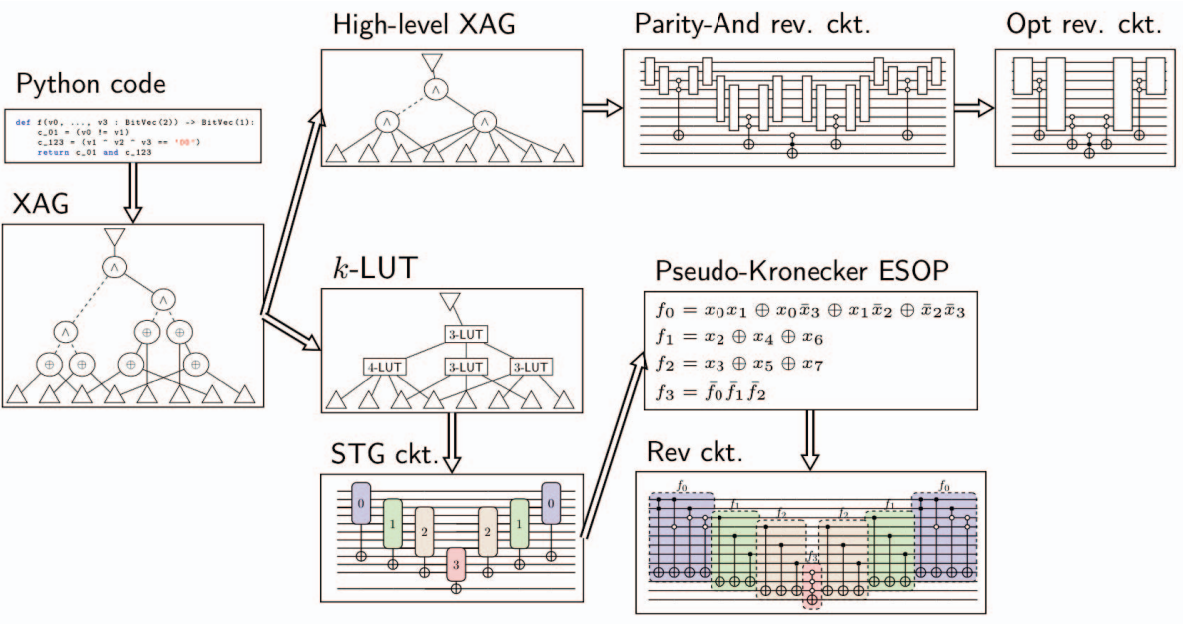
\includegraphics[width=0.7\textwidth]{figure/boolean.png}
    \caption{overview of possible Boolean function synthesis flows} 
    \label{fig-boolean}
  \end{figure}
\end{frame}
\begin{frame}{compilation passes}
  \begin{itemize}
    \item 
  \end{itemize}
\end{frame}
